\subsection{Best-First Search}

Breadth-first and depth-first search are examples of the more generic \emph{best-first} search algorithm, in which the frontier node visited next is that with the lowest estimated solution cost, given by an evaluation function \( \function{f}{\text{node}} \).
For breadth-first search, the estimated solution cost of a node is its depth; shallower nodes are visited first.
For depth-first search, the estimated solution cost is the negative of the depth; deeper nodes are visited first.

In order to improve efficiency over uninformed search algorithms, \emph{informed} search algorithms use problem-specific knowledge beyond what is included in the problem formulation.
Commonly, this knowledge takes the form of a \emph{heuristic} function \( \function{h}{\text{node}} \) that maps a node to the estimated cost of the cheapest path from its state to a goal state.
This is used as a guide in order to reduce the number of node expansions required in order to find a goal state.

Since the use of a heuristic function is intended to improve efficiency, it must be simple and quick to compute.
Thus, heuristics are approximate and not guaranteed to work.
For example, in the problem of finding a route between an origin and a destination, following existing paths between cities, a useful heuristic may be the straight-line distance of each city from the destination.
The increase in efficiency over the uninformed search is dependent on the quality of the heuristic.

\subsection{A* Search}

The \emph{A* search} is a popular best-first informed search algorithm that can be used to solve problems in which the costs of actions may differ.
Its evaluation function \( \function{f}{\text{node}} \) is the sum of the costs of the actions taken to reach the current node \( \function{g}{\text{node}} \) and a heuristic function \( \function{h}{\text{node}} \).
\begin{equation*}
  \function{f}{\text{node}} = \function{g}{\text{node}} + \function{h}{\text{node}}
\end{equation*}

To perform an A* search
\begin{enumerate}
  \item visit the frontier node with the smallest \( \function{f}{\text{node}} \) first, placing its children in the frontier, but
  \item do not place a child in the frontier if its corresponding state is represented by a node already in the list of visited nodes, and
  \item if the state of a child is represented by a node already in the frontier, and the node already in the frontier has a larger \( \function{g}{\text{node}} \), remove it and add the new child node to the frontier.
  \item Stop searching when a goal node is visited.
\end{enumerate}

In order to find the optimal solution, it is necessary that the search only terminates in success when a goal node is visited.

A heuristic is \emph{consistent} if the heuristic cost from any node to a goal node is less than or equal to the sum of the actual cost from the node to any other node and the heuristic cost from that node to the goal.
Thus, a consistent heuristic gives an underestimate rather than an overestimate.
\begin{equation*}
  \function{h}{n} \leq \function{\text{cost}}{n, n'} + \function{h}{n'}
\end{equation*}

\begin{figure}[htp]
  \centering
  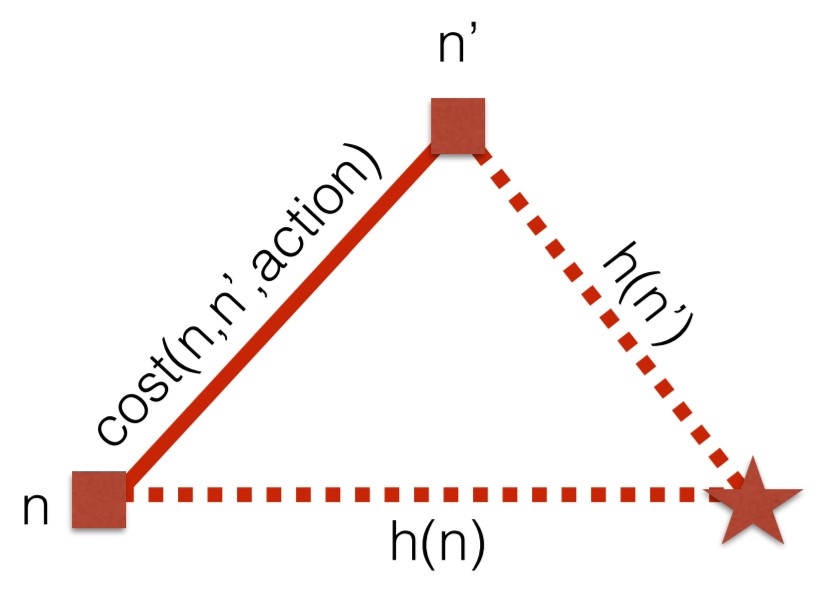
\includegraphics[width=0.3\textwidth]{unit-9/figures/heuristic-consistency.jpg}
  \caption*{The consistency of a heuristic.}
\end{figure}

An A* search has the following properties.
\begin{itemize}
  \item It is complete for any consistent heuristic --- if the heuristic is consistent, the search is guaranteed to find a path to a goal state if one exists, or to terminate in failure otherwise.
  \item It is optimal for any consistent heuristic --- if the heuristic is consistent, the search is guaranteed to find the shortest path to a goal state.
  \item It is optimally efficient for any consistent heuristic --- no other optimal search algorithm using the same heuristic is guaranteed to expand fewer nodes.
\end{itemize}

The time and space complexities of the A* search depend on the state space.
Usually, they are exponential in the depth \( d \) of the optimal solution and in the relative error \( e \) of the heuristic (\( \function{O}{b^{ed}} \)).
\begin{equation*}
  e = \frac{\text{actual cost} - \text{heuristic cost}}{\text{actual cost}}
\end{equation*}
A good heuristic is able to reduce space and time complexity considerably in comparison to an uninformed search.
A heuristic that has a small relative error \( e \), or that can effectively reduce the branch factor \( b \) close to one, will produce very large savings.

In order to improve efficiency, a heuristic can be designed that is more accurate, but not strictly consistent.
In this case, it may be possible to find a good solution without expanding as many nodes, but the solution is not guaranteed to be optimal.

One disadvantage of A* search is that heuristics are problem-specific and can be difficult to devise.
A good idea is to base the heuristic on a relaxed version of the problem --- one with fewer restrictions on actions.
For example, a relaxed version of the sliding tile puzzle may allow tiles to move over other tiles.
A possible heuristic for a state of the puzzle  is the sum of the Manhattan distances between each tile and its goal position.

The A* search algorithm can be applied to any graph-traversal problem.
It is often used for path-finding in video games.
